\chapter{Literature Review and Related Work}
\label{chap:relatedworks}



\section{Competitor Analysis}
\label{section:competitor-analysis}

% //#TODO: place table here
% \begin{figure}[h]
%     \centering
%     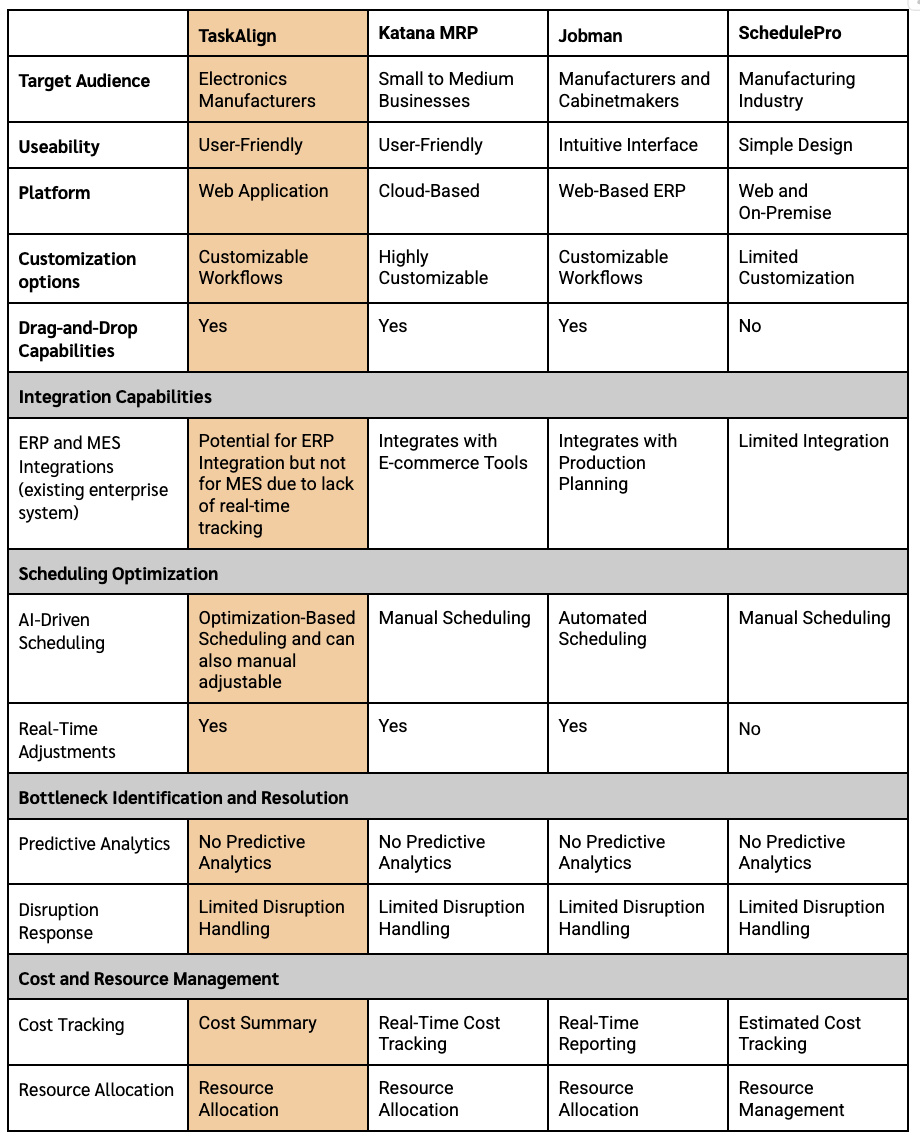
\includegraphics[width=0.5\textwidth]{examples/competitor.png}
%     \caption{Competitor Analysis Table} 
% \end{figure}

% Please add the following required packages to your document preamble:
% Beamer presentation requires \usepackage{colortbl} instead of \usepackage[table,xcdraw]{xcolor}

% Please add the following required packages to your document preamble:
% \usepackage[table,xcdraw]{xcolor}
% Beamer presentation requires \usepackage{colortbl} instead of \usepackage[table,xcdraw]{xcolor}

\begin{table}[h]
    \centering
    \renewcommand{\arraystretch}{1.3} % Adjust row height
    \setlength{\tabcolsep}{3pt} % Adjust column width
    \caption{Competitor Analysis}
    \resizebox{\textwidth}{!}{
    \begin{tabular}{|p{4cm}|p{4cm}|p{4cm}|p{4cm}|p{4cm}|}
        \hline
        & \textbf{TaskAlign} & \textbf{Katana MRP} & \textbf{Jobman} & \textbf{SchedulePro} \\
        \hline
        \textbf{Target Audience} & Electronics Manufacturers & Small to Medium Businesses & Manufacturers and Cabinetmakers & Batch and Semi-Continuous Manufacturing \\
        \hline
        \textbf{Platform} & Web Application & Cloud-Based & Web-Based ERP & Web and On-Premise \\
        \hline
        \textbf{Customization Options} & Customizable Workflows & Highly Customizable & Customizable Workflows & Limited Customization \\
        \hline
        \textbf{Drag-and-Drop Capabilities} & Yes & No Information & Yes & No \\
        \hline
        \textbf{Integration Capabilities} & ERP and MES Integrations (existing enterprise system) & Potential for ERP Integration but not for MES due to lack of real-time tracking & Integrates with E-commerce Tools & Integrates with Production Planning, Limited Integration \\
        \hline
        \textbf{Scheduling Optimization} & AI-Driven Scheduling & Optimization-Based Scheduling and can also be manually adjusted & Manual Scheduling & Automated Scheduling, Manual Scheduling \\
        \hline
        \textbf{Real-Time Adjustment} & No & Yes & Yes & No \\
        \hline
        \textbf{Bottleneck Identification and Resolution} & Predictive Analytics & No Predictive Analytics & Comes with Manufacturing Analytics & No Predictive Analytics, Statistical Analytics \\
        \hline
        \textbf{Cost and Resource Management} & Cost Tracking & Cost Summary & Real-Time Cost Tracking & Estimated Cost Tracking \\
        \hline
        \textbf{Resource Allocation} & Resource Allocation & Resource Management & Resource Allocation & Resource Management \\
        \hline
    \end{tabular}}
    \label{tab:competitor-analysis}
\end{table}


TaskAlign is a task scheduling system tailored for conventional electronics equipment factories reliant on manual production management. It empowers factory managers and operators to design optimized job schedules based on user-defined criteria, such as production time, machine utilization, and workforce allocation. The system considers constraints like machine cool-down time, energy consumption, and production dependencies. TaskAlign employs a data encoding system to translate user inputs (e.g. machine specifications, worker assignments, product requirements, dependencies) into a structured factory workflow representation suitable for optimization algorithms. These algorithms generate an optimal production schedule, maximizing machine utilization and workforce allocation while respecting constraints. Users can view and adjust schedules via Gantt charts and timelines, allowing for manual refinement of production plans. While TaskAlign does not provide real-time schedule adjustments, its optimization-based scheduling and customizable workflows offer a powerful solution for electronics manufacturers.

\subsection{Competitor Overview}

\textbf{Katana MRP}: Katana MRP is a cloud-based manufacturing ERP designed for small to medium-sized businesses. Its strengths lie in sales order fulfillment and inventory management, featuring e-commerce integration and real-time cost tracking. Katana MRP also provides manufacturing analytics and ERP and MES integrations. However, its manual scheduling approach and lack of drag-and-drop capabilities may limit its suitability for manufacturers requiring more dynamic production control \cite{katana_mrp}.

\textbf{Jobman}: Jobman is a web-based ERP solution designed for manufacturers and cabinetmakers. It includes production planning and real-time cost reporting. While Jobman offers automated scheduling and customizable workflows, it lacks predictive analytics and has limited integration capabilities, which may not fully address the needs of electronics manufacturers with complex workflows and existing enterprise systems \cite{jobman_erp}.

\textbf{SchedulePro}: SchedulePro is a scheduling software aimed at batch and semi-continuous manufacturing, offering a simple design and on-premise deployment. It provides statistical analytics and resource management features to improve production efficiency. However, its manual scheduling approach, limited customization options, and lack of integration capabilities may not meet the flexibility and connectivity needs of electronics manufacturers looking for comprehensive scheduling optimization \cite{schedulepro}.

\subsection{How TaskAlign Addresses Competitor Shortcomings}
TaskAlign distinguishes itself by catering specifically to the electronics manufacturing sector, offering optimization-based scheduling and cost summaries. Unlike Katana MRP, TaskAlign prioritizes resource allocation optimization. While Jobman provides automated scheduling, TaskAlign offers customizable scheduling tailored to electronics production, including drag-and-drop capabilities for further optimization. In contrast to SchedulePro's limited customization, TaskAlign provides highly adaptable workflows, enabling electronics manufacturers to tailor the system to their unique processes. Although TaskAlign does not offer real-time schedule adjustments, it has the potential to integrate with ERP systems, enhancing overall production management.


\section{Literature Review}
\label{section:literature-review}

Job scheduling optimization is a critical aspect of manufacturing systems, particularly in environments with complex constraints and dynamic requirements. This section reviews three key studies that contribute to advancements in this field.

\subsection{Optimization Model for Production Scheduling Considering Preventive Maintenance}
In the dynamic environment of Industry 4.0, \cite{optimization2023} proposed a mathematical optimization model for production scheduling that integrates preventive maintenance activities. The model accounts for real-life constraints such as machine downtime, scrap/rework, availability of raw materials, legal overtime limits, and transit times. It aims to create valid production schedules by distributing production orders across available machines while considering constraints like machine capacity, productivity norms, and planned maintenance. The model also allows for timely adjustments to handle uncertainties effectively. Verification was conducted through quasi-real and real-life experiments using data from an automotive manufacturer of locking systems. Results demonstrated the model's ability to optimize production schedules while accommodating preventive maintenance requirements.

\subsection{Data-Mining-Based Real-Time Optimization of Job Shop Scheduling}
\cite{datamining2022} explored real-time optimization techniques for job shop scheduling problems using data-mining approaches. The study focused on the dynamic nature of job shop environments where real-time data is critical for decision-making. By leveraging historical and real-time data, the proposed method identifies patterns and optimizes scheduling decisions dynamically. The approach integrates machine learning algorithms to predict job completion times and adjust schedules accordingly. Experimental results showed improvements in scheduling efficiency, reduced idle times, and enhanced resource utilization compared to traditional methods. This study highlights the importance of integrating data-driven techniques into job shop scheduling optimization.

\subsection{Multi-Objective Optimal Scheduling with Labor Workload Balance}
\cite{multiobjective2021} addressed multi-objective scheduling problems by considering labor workload distribution alongside traditional objectives like minimizing makespan or maximizing machine utilization. The proposed model balances workload distribution among workers while optimizing production schedules. It incorporates constraints related to worker availability, skill levels, and fatigue thresholds to ensure equitable workload distribution. The study used metaheuristic algorithms such as Genetic Algorithms (GAs) and Particle Swarm Optimization (PSO) to solve the problem efficiently. Experimental results demonstrated significant improvements in both workload balance and overall production efficiency, making it a promising approach for human-centric manufacturing systems.

\subsection{Conclusion}
These studies collectively demonstrate the potential of integrating mathematical models, data-driven techniques, and multi-objective optimization into job scheduling strategies. They provide valuable insights into addressing practical constraints such as preventive maintenance, real-time adaptability, and labor workload balance.
